\section{The derivative function} \label{S:2.2.DerivativeFxn}

\begin{goals}
\item How does the limit definition of the derivative of a function $f$ lead to an entirely new (but related) function $f'$?
\item What is the difference between writing $f'(a)$ and $f'(x)$?
\item How is the graph of the derivative function $f'(x)$ connected to the graph of $f(x)$?
\item What are some examples of functions $f$ for which $f'$ is not defined at one or more points?
\item What does it mean graphically to say that a function $f$ is differentiable at $x = a$?  How is this connected to the function being locally linear? 
\end{goals}

%--------------------------------------
% SUBSECTION INTRODUCTION
%--------------------------------------
\subsection*{Introduction}

Given a function $y = f(x)$, we now know that if we are interested in the instantaneous rate of change of the function at $x = a$, or equivalently the slope of the tangent line to $y = f(x)$ at $x = a$, we can compute the value $f'(a)$.  In all of our examples to date, we have arbitrarily identified a particular value of $a$ as our point of interest: $a = 1$, $a = 3$, etc.  But it is not hard to imagine that we will often be interested in the derivative value for more than just one $a$-value, and possibly for many of them.  In this section, we explore how we can move from computing simply $f'(1)$ or $f'(3)$ to working more generally with $f'(a)$, and indeed $f'(x)$.  Said differently, we will work toward understanding how the so-called process of "taking the derivative" generates a new function that is derived from the original function $y = f(x)$.  The following preview activity starts us down this path.

\begin{pa} \label{PA:1.4}
Consider the function $f(x) = 4x - x^2$.
\ba
	\item Use the limit definition to compute the following derivative values:  $f'(0)$, $f'(1)$, $f'(2)$, and $f'(3)$.
	\item Observe that the work to find $f'(a)$ is the same, regardless of the value of $a$.  Based on your work in (a), what do you conjecture is the value of $f'(4)$?  How about $f'(5)$?  (Note: you should \emph{not} use the limit definition of the derivative to find either value.)
	\item Conjecture a formula for $f'(a)$ that depends only on the value $a$.  That is, in the same way that we have a formula for $f(x)$ (recall $f(x) = 4x - x^2$), see if you can use your work above to guess a formula for $f'(a)$ in terms of $a$.
\ea
\end{pa} \afterpa % PREVIEW ACTIVITY

%-----------------------------------
% SUBSECTION DERIVATIVE FUNCTION
%-----------------------------------
\subsection*{How the derivative is itself a function}

In your work in Preview Activity~\ref{PA:1.4} with $f(x) = 4x - x^2$, you may have found several patterns.  One comes from observing that $f'(0) = 4$, $f'(1) = 2$, $f'(2) = 0$, and $f'(3) = -2$.  That sequence of values leads us naturally to conjecture that $f'(4) = -4$ and $f'(5) = -6.$  Even more than these individual numbers, if we consider the role of $0$, $1$, $2$, and $3$ in the process of computing the value of the derivative through the limit definition, we observe that the particular number has very little effect on our work.  To see this more clearly, we compute $f'(a)$, where $a$ represents a number to be named later.  Following the now standard process of using the limit definition of the derivative, 
\begin{eqnarray*}
f'(a) & = & \lim_{h \to 0} \frac{f(a + h) - f(a)}{h} \\
& = & \lim_{h \to 0} \frac{4(a + h) - (a + h)^2 - (4a-a^2)}{h} \\
& = & \lim_{h \to 0} \frac{4a + 4h - a^2 - 2ha - h^2 - 4a+a^2}{h} \\
& = & \lim_{h \to 0} \frac{4h - 2ha - h^2}{h} \\
& = & \lim_{h \to 0} \frac{h(4 - 2a - h)}{h} \\
& = & \lim_{h \to 0} (4 - 2a - h).
\end{eqnarray*}
Here we observe that neither $4$ nor $2a$ depend on the value of $h$, so as $h \to 0$, $(4 - 2a - h) \to (4 - 2a)$.  Thus, $f'(a) = 4 - 2a$.

This observation is consistent with the specific values we found above:  e.g., $f'(3) = 4 - 2(3) = -2$.  And indeed, our work with $a$ confirms that while the particular value of $a$ at which we evaluate the derivative affects the value of the derivative, that value has almost no bearing on the process of computing the derivative.   We note further that the letter being used is immaterial:  whether we call it $a$, $x$, or anything else, the derivative at a given value is simply given by ``$4$ minus $2$ times the value.''  We choose to use $x$ for consistency with the original function given by $y = f(x)$, as well as for the purpose of graphing the derivative function, and thus we have found that for the function $f(x) = 4x - x^2$, it follows that $f'(x) = 4 - 2x.$

\begin{marginfigure} % MARGIN FIGURE
\margingraphics{figures/1_4_ffprimeplot.eps} %figure 1.18 Active
\caption{The graphs of $f(x) = 4x - x^2$ (at left) and $f'(x) = 4 - 2x$ (at right).  Slopes on the graph of $f$ correspond to heights on the graph of $f'$.}
\label{fig:2-2_ffprime}
\end{marginfigure}

Because the value of the derivative function is so closely linked to the graphical behavior of the original function, it makes sense to look at both of these functions plotted on the same domain.  In Figure~\ref{fig:2-2_ffprime}, on the left we show a plot of $f(x) = 4x - x^2$ together with a selection of tangent lines at the points we've considered above.  On the right, we show a plot of $f'(x) = 4 - 2x$ with emphasis on the heights of the derivative graph at the same selection of points.  Notice the connection between colors in the left and right graph:  the green tangent line on the original graph is tied to the green point on the right graph in the following way:  \emph{the slope of the tangent line} at a point on the left-hand graph is the same as the \emph{height} at the corresponding point on the right-hand graph.  That is, at each respective value of $x$, the slope of the tangent line to the original function at that $x$-value is the same as the height of the derivative function at that $x$-value.  Do note, however, that the units on the vertical axes are different:  in the left graph, the vertical units are simply the output units of $f$.  On the right-hand graph of $y = f'(x)$, the units on the vertical axis are units of $f$ per unit of $x$.

\marginnote{Of course, this relationship between the graph of a function $y = f(x)$ and its derivative is a dynamic one.  An excellent way to explore how the graph of $f(x)$ generates the graph of $f'(x)$ is through a java applet.  See, for instance, the applets at \href{http://gvsu.edu/s/5C}{\texttt{http://gvsu.edu/s/5C}} or \href{http://gvsu.edu/s/5D}{\texttt{http://gvsu.edu/s/5D}}, via the sites of David Austin(\href{http://gvsu.edu/s/5r}{\texttt{http://gvsu.edu/s/5r}}) and Marc Renault(\href{http://gvsu.edu/s/5p}{\texttt{http://gvsu.edu/s/5p}}).}

In Section~\ref{S:2.1.DerivativePt} when we first defined the derivative, we wrote the definition in terms of a value $a$ to find $f'(a)$.  As we have seen above, the letter $a$ is merely a placeholder, and it often makes more sense to use $x$ instead.  For the record, here we restate the  definition of the derivative\index{derivative!definition}.

\definition{Derivative as a Function}{ %DEFINITION
Let $f$ be a function and $x$ a value in the function's domain.  We define the \emph{derivative of $f$ with respect to $x$ at the value $x$}, denoted $f'(x)$, by the formula
$\ds f'(x) = \lim_{h \to 0} \frac{f(x+h)-f(x)}{h},$
provided this limit exists. \\

\noindent\textbf{Notation:} 
Let $y = f(x)$. The following notation all represents the derivative:
\[ f'(x) = y' = \frac{dy}{dx} = \frac{df}{dx} = \frac{d}{dx}(f) = \frac{d}{dx}(y). \]
} % end definition

\marginnote{\textbf{Important:} The notation $\ds \frac{dy}{dx}$ is one symbol; it is \textbf{not} the fraction ``$dy/dx$''. The notation, while somewhat confusing at first, was chosen with care. A fraction--looking symbol was chosen because the derivative has many fraction--like properties. Among other places, we see these properties at work when we talk about the units of the derivative, when we discuss the Chain Rule, and when we learn about integration (topics that appear in later sections and chapters)}

We now may take two different perspectives on thinking about the derivative function:  given a graph of $y = f(x)$, how does this graph lead to the graph of the derivative function $y = f'(x)$?  and given a formula for $y = f(x)$, how does the limit definition of the derivative generate a formula for $y = f'(x)$?  We first explore the graphical relationship in the following activity. 

\begin{activity} \label{A:2.2.1}
For each given graph of $y = f(x)$, sketch an approximate graph of its derivative function, $y = f'(x)$, on the axes immediately below.  The scale of the grid for the graph of $f$ is $1 \times 1$; assume the horizontal scale of the grid for the graph of $f'$ is identical to that for $f$.  If necessary, adjust and label the vertical scale on the axes for the graph of $f'$.

Write several sentences that describe your overall process for sketching the graph of the derivative function, given the graph the original function.  What are the values of the derivative function that you tend to identify first?  What do you do thereafter?  How do key traits of the graph of the derivative function exemplify properties of the graph of the original function?
\end{activity}

\begin{adjustwidth*}{}{-.855in}
\begin{center}
\includegraphics{figures/1_4_Act1a.eps} 
\centerline{\hspace{4in}}
\includegraphics{figures/1_4_Act1b.eps}
\end{center}
\end{adjustwidth*}

\begin{center}
\includegraphics{figures/1_4_Act1c.eps}
\centerline{\hspace{4in}}
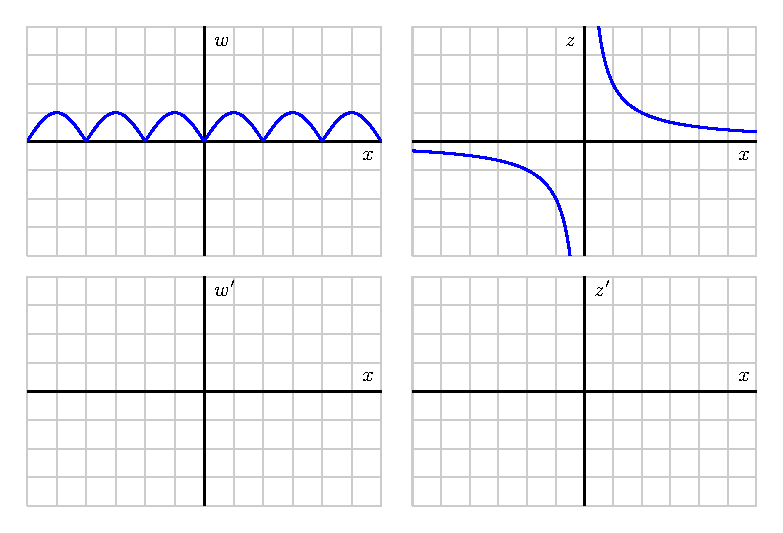
\includegraphics{figures/1_4_Act1d.eps}
\end{center}


\begin{smallhint}
Points where the slope of the tangent line is equal to zero are particularly important.  Try finding these points first in your effort to plot $y = f'(x)$ and plotting those zero values on the axes where you'll graph $y = f'(x)$.  
\end{smallhint}
\begin{bighint}
Points where the slope of the tangent line is equal to zero are particularly important.  Try finding these points first in your effort to plot $y = f'(x)$ and plotting those zero values on the axes where you'll graph $y = f'(x)$.  After doing so, think carefully as well about the questions: at this point, is $f'(x)$ positive or negative?  is $f'(x)$ big or small.  Use these ideas to help you sketch the derivative graph for the following functions.
\end{bighint}
\begin{activitySolution}
\begin{center}
\includegraphics{figures/1_4_Act1aSoln.eps} \\
\underline{\hspace{4in}}\\
\ \\
\includegraphics{figures/1_4_Act1bSoln.eps}
\end{center}

\begin{center}
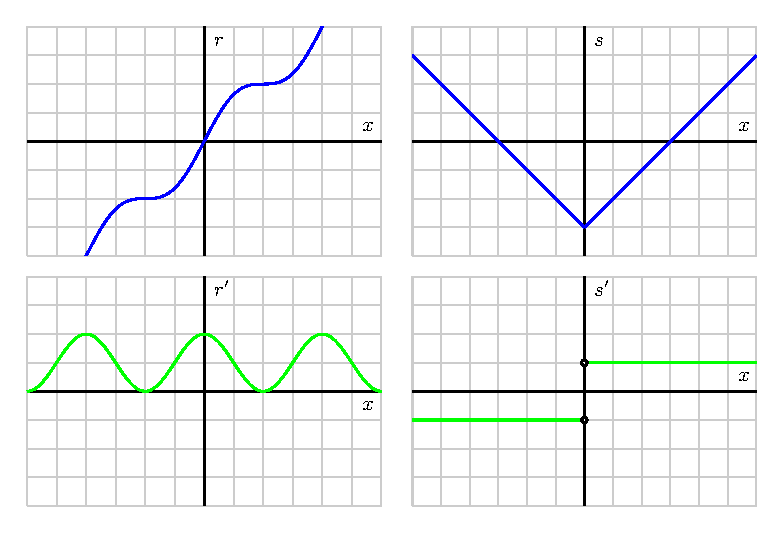
\includegraphics{figures/1_4_Act1cSoln.eps} \\
\underline{\hspace{4in}}\\
\ \\
\includegraphics{figures/1_4_Act1dSoln.eps}
\end{center}
\end{activitySolution}
\aftera % ACTIVITY 

\marginnote{For a dynamic investigation that allows you to experiment with graphing $f'$ when given the graph of $f$, see \href{http://gvsu.edu/s/8y}{\texttt{http://gvsu.edu/s/8y}}.(Source: Marc Renault, Calculus Applets Using Geogebra.)} 

Now, recall the opening example of this section:  we began with the function $y = f(x) = 4x - x^2$ and used the limit definition of the derivative to show that $f'(a) = 4 - 2a$, or equivalently that $f'(x) = 4 - 2x$.  We subsequently graphed the functions $f$ and $f'$ as shown in Figure~\ref{fig:2-2_ffprime}.  Following Activity~\ref{A:2.2.1}, we now understand that we could have constructed a fairly accurate graph of $f'(x)$ \emph{without} knowing a formula for either $f$ or $f'$.  At the same time, it is ideal to know a formula for the derivative function whenever it is possible to find one.

\begin{example} \label{Ex:2.2.Eg1}
Let $f(x) = 3x^2+5x-7$. Find $f'(x)$.

\solution We apply the definition of the derivative.
\begin{align*}
f'(x) &= \lim_{h \to 0} \frac{f(x+h)-f(x)}{h} \\
&=	\lim_{h \to 0} \frac{3(x+h)^2+5(x+h)-7-(3x^2+5x-7)}{h}\\
&=	\lim_{h \to 0} \frac{3h^2 +6xh+5h}{h}\\
&= \lim_{h \to 0} 3h+6x+5 \\
&= 6x+5
\end{align*}
So $f'(x) = 6x+5$. Recall in Example~\ref{Ex:2.1.Eg2} of Section~\ref{S:2.1.DerivativePt}, we found that $f'(1) = 11$ and $f'(3) = 23$. Note our new computation of $f'(x)$ affirm these facts.
\end{example}

 % EXAMPLE

\begin{example} \label{Ex:2.2.Eg2}
Let $\ds f(x) = \frac{1}{x+1}$. Find $f'(x)$.

\solution We again apply the definition of the derivative.
\begin{align*}
f'(x) &= \lim_{h \to 0} \frac{f(x+h)-f(x)}{h}\\
&=	\lim_{h\to 0} \frac{\frac{1}{x+h+1}-\frac{1}{x+1}}{h} \intertext{Now find a common denominator then subtract; pull $1/h$ out front to facilitate reading.}
&= \lim_{h\to 0} \frac{1}{h}\cdot\left(\frac{x+1}{(x+1)(x+h+1)} - \frac{x+h+1}{(x+1)(x+h+1)}\right)\\
&=	\lim_{h\to 0} \frac 1h\cdot\left(\frac{x+1-(x+h+1)}{(x+1)(x+h+1)}\right)\\
&=	\lim_{h\to 0} \frac1h\cdot\left(\frac{-h}{(x+1)(x+h+1)}\right)\\
&=	\lim_{h\to 0} \frac{-1}{(x+1)(x+h+1)} \\
&= \frac{-1}{(x+1)(x+1)}\\
&= \frac{-1}{(x+1)^2}
\end{align*}
	
So $\ds f'(x) = \frac{-1}{(x+1)^2}$. To practice our notation, we could also state 
\[ \ds \frac{d}{dx}\left(\frac{1}{x+1}\right) = \frac{-1}{(x+1)^2}. \]
\end{example}

 %EXAMPLE

In the next activity, we further explore the more algebraic approach to finding $f'(x)$:  given a formula for $y = f(x)$, the limit definition of the derivative will be used to develop a formula for $f'(x)$.  

\begin{activity} \label{A:2.2.2}
For each of the listed functions, determine a formula for the derivative function.  For the first two, determine the formula for the derivative by thinking about the nature of the given function and its slope at various points; do not use the limit definition.  For the latter four, use the limit definition.  Pay careful attention to the function names and independent variables.  It is important to be comfortable with using letters other than $f$ and $x$.  For example, given a function $p(z)$, we call its derivative $p'(z)$.
\begin{multicols}{3}
\ba
	\item $\ds (x) = 1$
	\item $\ds g(t) = t$
	\item $\ds p(z) = z^2$
	\item $\ds q(s) = s^3$
	\item $\ds F(t) = \frac{1}{t}$
	\item $\ds G(y) = \sqrt{y}$
\ea
\end{multicols}

\end{activity}
\begin{smallhint}
\ba
	\item  What is the slope of the function at every point?
	\item  What is the slope of the function at every point?
	\item  $p(z+h) = (z+h)^2$
	\item  $q(s+h) = (s+h)^3$
	\item  $F(t+h) = \frac{1}{t+h}$
	\item  $G(y+h) = \sqrt{y+h}$
\ea
\end{smallhint}
\begin{bighint}
\ba
	\item  The function is a horizontal line.
	\item  The function is a line with slope 1.
	\item  $p(z+h) - p(z) = (z+h)^2 - z^2 = z^2 + 2zh + h^2 - z^2$
	\item  $q(s+h) - q(s) = (s+h)^3 - s^3 = s^3 + 3s^2h + 3sh^2 + h^3 - s^3$
	\item  Find a common denominator for $ \frac{1}{t+h} - \frac{1}{t}$.
	\item  Multiply the difference quotient by this form of 1: $\frac{\sqrt{y+h} + \sqrt{y}}{\sqrt{y+h} + \sqrt{y}}.$
\ea
\end{bighint}
\begin{activitySolution}
\ba
	\item  $f'(x) = 0$ because the slope of the tangent line to the horizontal line given by $f(x) = 1$ is zero at every value of $x$.
	\item  $g'(t) = 1$ because the slope of the tangent line to the line given by $g(t) = t$ is 1 at every value of $t$.
	\item  \begin{eqnarray*}
		p'(z) & = & \lim_{h \to 0} \frac{p(z+h) - p(z)}{h} \\
		       & = & \lim_{h \to 0} \frac{(z+h)^2 - z^2}{h} \\
		       & = & \lim_{h \to 0} \frac{z^2 + 2zh + h^2 - z^2}{h} \\
		       & = & \lim_{h \to 0} \frac{2zh + h^2}{h} \\
		       & = & \lim_{h \to 0} 2z + h \\
		       & = & 2z
		 \end{eqnarray*}
		 
	\item  \begin{eqnarray*}
		q'(s) & = & \lim_{h \to 0} \frac{q(s+h) - q(s)}{h} \\
		       & = & \lim_{h \to 0} \frac{(s+h)^3 - s^3}{h} \\
		       & = & \lim_{h \to 0} \frac{s^3 + 3s^2h + 3sh^2 + h^3 - s^3}{h} \\
		       & = & \lim_{h \to 0} \frac{3s^2h + 3sh^2 + h^2}{h} \\
		       & = & \lim_{h \to 0} 3s^2 + 3sh + h \\
		       & = & 3s^2
		 \end{eqnarray*}
	\item  \begin{eqnarray*}
		F'(t) & = & \lim_{h \to 0} \frac{F(t+h) - F(s)}{h} \\
		       & = & \lim_{h \to 0} \frac{\frac{1}{t+h} - \frac{1}{t}}{h} \\
		       & = & \lim_{h \to 0} \frac{\frac{t - (t+h)}{t(t+h)}}{h} \\
		       & = & \lim_{h \to 0} \frac{-h}{ht(t+h)} \\
		       & = & \lim_{h \to 0} \frac{-1}{t(t+h)} \\
		       & = & \frac{-1}{t^2}
		 \end{eqnarray*}
	\item  \begin{eqnarray*}
		G'(y) & = & \lim_{h \to 0} \frac{G(y+h) - G(y)}{h} \\
		       & = & \lim_{h \to 0} \frac{\sqrt{y+h}-\sqrt{y}}{h} \\
		       & = & \lim_{h \to 0} \frac{\sqrt{y+h}-\sqrt{y}}{h} \cdot \frac{\sqrt{y+h} + \sqrt{y}}{\sqrt{y+h} + \sqrt{y}} \\
		       & = & \lim_{h \to 0} \frac{(y+h)-y}{h(\sqrt{y+h} + \sqrt{y})} \\
		       & = & \lim_{h \to 0} \frac{h}{h(\sqrt{y+h} + \sqrt{y})} \\
		       & = & \lim_{h \to 0} \frac{1}{\sqrt{y+h} + \sqrt{y}} \\
		       & = & \frac{1}{2\sqrt{y}}
		 \end{eqnarray*}		 
\ea
\end{activitySolution}
\aftera % ACTIVITY 

%-------------------------------------------
% SUBSECTION DIFFERENTIABILITY
%-------------------------------------------
\subsection*{Differentiability}

We recall that a function $f$ is said to be differentiable at $x = a$ whenever $f'(a)$ exists.  Moreover, for $f'(a)$ to exist, we know that the function $y = f(x)$ must have a tangent line at the point $(a,f(a))$, since $f'(a)$ is precisely the slope of this line.  In order to even ask if $f$ has a tangent line at $(a,f(a))$, it is necessary that $f$ be continuous at $x = a$: if $f$ fails to have a limit at $x = a$, if $f(a)$ is not defined, or if $f(a)$ does not equal the value of $\ds \lim_{x \to a} f(x)$, then it doesn't even make sense to talk about a tangent line to the curve at this point.

Indeed, it can be proved formally that if a function $f$ is differentiable at $x = a$, then it must be continuous at $x = a$.  So, if $f$ is not continuous at $x = a$, then it is automatically the case that $f$ is not differentiable there.  For example, in Figure~\ref{fig:1-3_Con} from our early discussion of continuity, both $f$ and $g$ fail to be differentiable at $x = 1$ because neither function is continuous at $x = 1$.  But can a function fail to be differentiable at a point where the function is continuous?

In Figure~\ref{F:1.7.NotDiff}, we consider the situation where a function has a sharp corner at a point.  For the pictured function $f$, we observe that $f$ is clearly continuous at $a = 1$, since $\ds\lim_{x \to 1} f(x) = 1 = f(1).$

\begin{marginfigure} % MARGIN FIGURE
\margingraphics{figures/1_7_NotDiff.eps}
\caption{A function $f$ that is continuous at $a = 1$ but not differentiable at $a = 1$; at right, we zoom in on the point $(1,1)$ in a magnified version of the box in the left-hand plot.} \label{F:1.7.NotDiff}
\end{marginfigure}

But the function $f$ in Figure~\ref{F:1.7.NotDiff} is not differentiable at $a = 1$ because $f'(1)$ fails to exist.  One way to see this is to observe that $f'(x) = -1$ for every value of $x$ that is less than $1$, while $f'(x) = +1$ for every value of $x$ that is greater than $1$.  That makes it seem that either $+1$ or $-1$ would be equally good candidates for the value of the derivative at $x = 1$.   Alternately, we could use the limit definition of the derivative to attempt to compute $f'(1)$, and discover that the derivative does not exist.  Finally, we can also see visually that the function $f$ in Figure~\ref{F:1.7.NotDiff} does not have a tangent line.  When we zoom in on $(1,1)$ on the graph of $f$, no matter how closely we examine the function, it will always look like a ``V'', and never like a single line, which tells us there is no possibility for a tangent line there.  

To make a more general observation, if a function does have a tangent line at a given point, when we zoom in on the point of tangency, the function and the tangent line should appear essentially indistinguishable\footnote{See, for instance, \href{http://gvsu.edu/s/6J}{\texttt{http://gvsu.edu/s/6J}} for an applet (due to David Austin, GVSU) where zooming in shows the increasing similarity between the tangent line and the curve.  }.  Conversely, if we have a function such that when we zoom in on a point the function looks like a single straight line, then the function should have a tangent line there, and thus be differentiable.  Hence, a function that is differentiable at $x = a$ will, up close, look more and more like its tangent line at $(a,f(a))$, and thus we say that a function is differentiable at $x = a$ is \emph{locally linear}. \index{locally linear}

\begin{marginfigure}[1.5cm] % MARGIN FIGURE
\captionsetup[subfigure]{labelformat=empty}
\subfloat{\margingraphics{figures/figabsolutevalue}}

\subfloat{\margingraphics{figures/figabsolutevalueprime}}
\caption{Above: The absolute value function, $f(x) = |x|$. Notice how the slope of the lines (and hence the tangent lines) abruptly changes at $x=0$. Below: A graph of the derivative of $f(x) = |x|$.}\label{fig:2-2_Eg3.1}
\end{marginfigure}

\begin{example} \label{Ex:2.2.Eg3}
Find the derivative of the absolute value function---see Figure~\ref{fig:2-2_Eg3.1}.
\[ f(x) = |x| = \left\{\begin{array}{cc} -x & x<0 \\ x & x\geq 0\end{array}.\right. \]

\solution We need to evaluate $\ds \lim_{h \to 0}\frac{f(x+h)-f(x)}{h}.$ As $f$ is piecewise--defined, we need to consider separately the limits when $x<0$ and when $x>0$. 

When $x<0$:
\begin{align*}
\frac{d}{dx}\big(-x\big) 	&= \lim_{h\to 0}\frac{-(x+h) - (-x)}{h} \\
&=	\lim_{h \to 0}\frac{-h}{h}\\
&=	\lim_{h \to 0}-1 \\
&=	-1.
\end{align*}
When $x>0$, a similar computation shows that $\ds \frac{d}{dx}\big( x \big) = 1$. \\

We need to also find the derivative at $x=0$. By the definition of the derivative at a point, we have 
\[ f'(0) = \lim_{h \to 0}\frac{f(0+h)-f(0)}{h}.\]
Since $x=0$ is the point where our function's definition switches from one piece to other, we need to consider left and right-hand limits. Consider the following, where we compute the left and right hand limits side by side.

\noindent\begin{minipage}[b]{.5\linewidth}
\begin{align*}
\lim_{h \to 0^-} \frac{f(0+h)-f(0)}{h} &= \\
\lim_{h \to 0^-} \frac{-h-0}{h} &= \\
\lim_{h \to 0^-} -1 & =-1
\end{align*}
\end{minipage}\rule{.5pt}{70pt}
\begin{minipage}[b]{.5\linewidth}
\begin{align*}
\lim_{h \to 0^+} \frac{f(0+h)-f(0)}{h} &= \\
\lim_{h \to 0^+} \frac{h-0}{h} &= \\
\lim_{h \to 0^+} 1 & =1
\end{align*}
\end{minipage}
%		
%		$$\begin{array}{ccccc}
%		\displaystyle \lim_{h\to0}\frac{f(0+h)-f(0)}{h} & = & \displaystyle\lim_{h\to0^-}\frac{f(0+h)-f(0)}{h} &=&\displaystyle\lim_{h\to0^+}\frac{f(0+h)-f(0)}{h}\\
%	\rule{0pt}{20pt}	&= & \displaystyle\lim_{h\to0^-}\frac{-h-0}{h} &=&\displaystyle\lim_{h\to0^+}\frac{h-0}{h}\\
%	\rule{0pt}{15pt}	&= & \displaystyle\lim_{h\to0^-}-1 &=&\displaystyle\lim_{h\to0^+}1\\
%	\rule{0pt}{12pt}	&= & -1 &=& 1\ !\\
%		\end{array}$$
%		
		
The last lines of each column tell the story: the left and right hand limits are not equal. Therefore the limit does not exist at $0$, and $f$ is not differentiable at $0$.
So we have 
\[ f'(x) = \left\{\begin{array}{cc} -1 & x<0 \\ 1 & x>0\end{array}.\right.\] 
At $x=0$, $f'(x)$ does not exist; there is a jump discontinuity at $0$; see Figure~\ref{fig:2-2_Eg3.1}. So $f(x) = |x|$ is differentiable everywhere except at $0$. 
\end{example}

 %EXAMPLE

\begin{marginfigure}[6cm]
\margingraphics{figures/1_7_PA1.eps}
\caption{The graph of $y = f(x)$ for Activity~\ref{A:2.2.3}.} \label{fig:2.2.Act3}
\end{marginfigure}

\begin{activity} \label{A:2.2.3} 
In this activity, we classify the points at which a function does not have a limit and is neither continuous nor differentiable.  Let $f$ be the function given in Figure~\ref{fig:2.2.Act3}.
\ba
\item State all values of $a$ for which $f$ does not have a limit at $x = a$.  For each, provide a reason for your conclusion.
\item State all values of $a$ for which $f$ is not continuous at $x = a$.  For each, provide a reason for your conclusion.
\item State all values of $a$ for which $f$ is not differentiable at $x = a$.  For each, provide a reason for your conclusion.
\item True or false: if a function $p$ is differentiable at $x = b$, then $\ds \lim_{x \to b} p(x)$ must exist.  Why?	
\ea

\end{activity}
\begin{smallhint}
\ba
	\item What type of function is $g$ for all $x < 0$?  For all $x > 0$?
	\item Recall that $g'(0) = \lim_{h \to 0} \frac{g(0 + h) - g(0)}{h}.$
	\item What is the value of $|h|$ when $h < 0$?
	\item You might start by identifying points where $f$ is not continuous.
	\item What does being differentiable at a point tell you about continuity there?	
\ea
\end{smallhint}
\begin{bighint}
\ba
	\item Think about how $g$ is a piecewise linear function.
	\item Recall that $g'(0) = \lim_{h \to 0} \frac{g(0 + h) - g(0)}{h}.$
	\item What is the value of $|h|$ when $h < 0$?  What does this tell you about $\frac{|h|}{h}$ when $h < 0$?
	\item Start by identifying points where $f$ is not continuous.  Then strive to identify any corner points.
	\item What does being differentiable at a point tell you about continuity at that point?	
\ea
\end{bighint}
\begin{activitySolution}
\ba
	\item We know that $g(x) = |x|$ is given by the formula $g(x) = -x$ when $x < 0$ and by $g(x) = x$ when $x \ge 0$.  Each of these pieces of $g$ is a straight line, so at every point other than the point where they meet, the function $g$ has a well-defined slope, and thus is differentiable. 
	\item Observe that
	\begin{eqnarray*}
		g'(0) & = & \lim_{h \to 0} \frac{g(0+h)-g(0)}{h} \\
			& = & \lim_{h \to 0} \frac{|0+h|-|0|}{h} \\
			& = & \lim_{h \to 0} \frac{|h|}{h}
	\end{eqnarray*}
	\item Following up on our work in (b), note that whenever $h > 0$, $|h| = h$, and thus
	$$\lim_{h \to 0^+} \frac{|h|}{h} = \lim_{h \to 0^+} \frac{h}{h} = 1,$$
	while whenever $h < 0$, $|h| = -h$, and thus
	$$\lim_{h \to 0^-} \frac{|h|}{h} = \lim_{h \to 0^-} \frac{-h}{h} = -1$$
	Since the right- and left-hand limits are not equal, it follows that 
	$$g'(0) =  \lim_{h \to 0} \frac{|h|}{h}$$
	does not exist.

	\item $f$ is not differentiable at $a = -2, -1, 2, 3$ because at each of these points $f$ is not continuous.  In addition, $f$ is not differentiable at $a = -3$ and $a = 1$ because the graph of $f$ has a corner point (or cusp) at each of these values.  
	\item True: if a function $p$ is differentiable at $x = b$, then $\lim_{x \to b} p(x)$ must exist.  This is true because we know that if $p$ is differentiable at a point, then $p$ is continuous there, and anytime a function is continuous at a point, it must have a limit there.	
\ea
\end{activitySolution}
\aftera % ACTIVITY This needs to now be redone!!

%--------------
% SUMMARY
%--------------
\begin{summary}
\item The limit definition of the derivative, $f'(x) = \lim_{h \to 0} \frac{f(x+h)-f(x)}{h}$, produces a value for each $x$ at which the derivative is defined, and this leads to a new function whose formula is $y = f'(x)$.  Hence we talk both about a given function $f$ and its derivative $f'$.  

\item There is essentially no difference between writing $f'(a)$ (as we did regularly in Section~\ref{S:2.1.DerivativePt}) and writing $f'(x)$.  In either case, the variable is just a placeholder that is used to define the rule for the derivative function.

\item Given the graph of a function $y = f(x)$, we can sketch an approximate graph of its derivative $y = f'(x)$ by observing that \emph{heights} on the derivative's graph correspond to \emph{slopes} on the original function's graph.

\item In this section, we encountered some functions that had sharp corners on their graphs, such as the shifted absolute value function.  At such points, the derivative fails to exist, and we say that $f$ is not differentiable there.  For now, it suffices to understand this as a consequence of the jump that must occur in the derivative function at a sharp corner on the graph of the original function.  
\end{summary}

%--------------
% EXERCISES
%--------------
\begin{adjustwidth*}{}{-2.25in}
\textbf{{\large Exercises}}
\setlength{\columnsep}{25pt}
\begin{multicols*}{2}
\noindent Terms and Concepts \small
\begin{enumerate}[1)]
\item {T/F: Let $f$ be a position function. The average rate of change on $[a,b]$ is the slope of the line through the points $(a, f(a))$ and $(b,f(b))$.}
\item {T/F: The definition of the derivative of a function at a point involves taking a limit.}
\item {In your own words, explain the difference between the average rate of change and instantaneous rate of change.}
\item Let $y = f(x)$. Give three different notations equivalent to ``$f'(x)$.''
\end{enumerate} 

\noindent {\normalsize Problems} \small

\noindent {\bf In exercises 5--8, a graph of a function is given. Using the graph, sketch $f'(x)$.}

\begin{enumerate}[1),resume]
\item \includegraphics[scale=.8]{figures/fig02_01_ex_26}
\item \includegraphics[scale=.8]{figures/fig02_01_ex_27}
\item \includegraphics[scale=.8]{figures/fig02_01_ex_28}
\item \includegraphics[scale=.8]{figures/fig02_01_ex_29}

\item Using the graph of $g(x)$ below, answer the following questions.
\ba
\item Where is $g(x) > 0$?
\item Where is $g(x) < 0$?
\item Where is $g(x) = 0$?
\item Where is $g'(x) < 0$?
\item Where is $g'(x) > 0$?
\item Where is $g'(x) = 0$?
\ea

\includegraphics[scale=.8]{figures/fig02_01_ex_30}

\item Let $f$ be a function with the following properties:  $f$ is differentiable at every value of $x$ (that is, $f$ has a derivative at every point), $f(-2) = 1$, and $f'(-2) = -2$, $f'(-1) = -1$, $f'(0) = 0$, $f'(1) = 1$, and $f'(2) = 2$.
\ba
	\item On the axes provided at left below, sketch a possible graph of $y = f(x)$.  Explain why your graph meets the stated criteria.
	\item On the axes at right below, sketch a possible graph of $y = f'(x)$.  What type of curve does the provided data suggest for the graph of $y = f'(x)$?
	\item Conjecture a formula for the function $y = f(x)$.  Use the limit definition of the derivative to determine the corresponding formula for $y = f'(x)$.  Discuss both graphical and algebraic evidence for whether or not your conjecture is correct.
\ea

\includegraphics[scale=.75]{figures/1_2_Ez3.eps} 
\end{enumerate}

%------------------------------------------
% END OF EXERCISES ON FIRST PAGE
%------------------------------------------
\end{multicols*}
\end{adjustwidth*}

\clearpage

\begin{adjustwidth*}{}{-2.25in}
\setlength{\columnsep}{25pt}
\begin{multicols*}{2}\small

\begin{enumerate}[1),start=11]
\item Let $g$ be a continuous function (that is, one with no jumps or holes in the graph) and suppose that a graph of $y= g'(x)$ is given by the graph on the right below.

\includegraphics[scale=.75]{figures/1_4_Ez2.eps} %\ \  \includegraphics{figures/1_2_Ez3.eps}

\ba
\item Observe that for every value of $x$ that satisfies $0 < x < 2$, the value of $g'(x)$ is constant.  What does this tell you about the behavior of the graph of $y = g(x)$ on this interval?
\item On what intervals other than $0 < x < 2$ do you expect $y = g(x)$ to be a linear function?  Why?
\item At which values of $x$ is $g'(x)$ not defined?  What behavior does this lead you to expect to see in the graph of $y=g(x)$?
\item Suppose that $g(0) = 1$.  On the axes provided at left, sketch an accurate graph of $y = g(x)$.
\ea

\item Consider the graph of the function $y = p(x)$ that is provided below on the left.  Assume that each portion of the graph of $p$ is a straight line, as pictured.

\includegraphics[scale=.75]{figures/1_7_Ez2.eps}

\ba
\item State all values of $a$ for which $\lim_{x \to a} p(x)$ does not exist.
\item State all values of $a$ for which $p$ is not continuous at $a$.
\item State all values of $a$ for which $p$ is not differentiable at $x = a$.
\item On the axes provided on the right, sketch an accurate graph of $y = p'(x)$.
\ea

\item For each of the following prompts, give an example of a function that satisfies the stated criteria.  A formula or a graph, with reasoning, is sufficient for each.  If no such example is possible, explain why.
\ba
\item A function $f$ that is continuous at $a = 2$ but not differentiable at $a = 2$.
\item A function $g$ that is differentiable at $a = 3$ but does not have a limit at $a=3$.
\item A function $h$ that has a limit at $a = -2$, is defined at $a = -2$, but is not continuous at $a = -2$.
\item A function $p$ that satisfies all of the following:
\begin{itemize}
\item $p(-1) = 3$ and $\ds\lim_{x \to -1} p(x) = 2$
\item $p(0) = 1$ and $p'(0) = 0$
\item $\ds\lim_{x \to 1} p(x) = p(1)$ and $p'(1)$ does not exist
\end{itemize}
\ea
\end{enumerate}

\vspace{.25cm}

\noindent {\bf For exercises 14--22, use the limit definition of the derivative to compute the derivative function.}

\bmtwo
\begin{enumerate}[1),resume]
\item $\ds f(x) = 8x$
\item $\ds y = x^2$
\item $\ds g(x) = 2x^2 + 3x$
\item $\ds s(t) = \frac{1}{\ds \sqrt{t}}$
\item $\ds r(x) = \frac{1}{x^2}$
\item $\ds f(x) = \ds\sqrt{3x-1}$
\item $\ds f(x) = \ds\sqrt{8x}$
\item $\ds s(t) = \frac{1}{t + 5}$
\item $\ds y = \frac{1}{2x - 1}$
\end{enumerate}
\emtwo

%------------------------------------------------
% END OF EXERCISES ON SECOND PAGE
%------------------------------------------------
\end{multicols*}
\end{adjustwidth*}
\afterexercises 

\cleardoublepage